\documentclass[11pt,a4paper]{article}
\usepackage[margin=27mm]{geometry}
\usepackage[T1]{fontenc}
\usepackage{lmodern}
\usepackage{amsmath,amssymb,amsthm}
\usepackage{booktabs,array}
\usepackage{tikz}
\usepackage{xcolor}
\usepackage[hidelinks]{hyperref}
\usepackage{microtype}
\usetikzlibrary{arrows.meta}
\newtheorem{theorem}{Theorem}[section]
\newtheorem{lemma}[theorem]{Lemma}
\newtheorem{proposition}[theorem]{Proposition}
\newtheorem{corollary}[theorem]{Corollary}
\theoremstyle{definition}
\newtheorem{definition}[theorem]{Definition}
\theoremstyle{remark}
\newtheorem{remark}[theorem]{Remark}
\newcommand{\V}{V}
\newcommand{\E}{E}
\newcommand{\NN}{N}
\newcommand{\Exp}{\mathcal{T}}
\newcommand{\palette}{(1,1,3,3,4)}
\newcommand{\weakpalette}{(1,1,3,3,3)}
\newcommand{\high}{\{A,B,C\}}
\DeclareMathOperator{\dist}{dist}
\title{A structural obstruction to\texorpdfstring{\\}{}\((1,1,3,3,4)\)-packing colorings}
\author{Author information pending confirmation}
\date{Private manuscript, version 0.1\\12 October 2026}

\begin{document}
\maketitle

\begin{abstract}
Mortada, El Zein and Al Hajjar asked whether every connected claw-free
subcubic graph, apart from their specified exception, admits a
\(\palette\)-packing coloring. We give a negative answer. For every odd
integer \(k\geq3\), the triangle expansion of a ring of \(k\) diamonds is
a connected cubic graph on \(12k\) vertices that admits no such coloring.
The proof selects an arbitrary existing high-colored vertex in each
triangle. The selected labels give a proper three-coloring of the core,
and the radius-four class forces an external private neighbor at each
of its core vertices. This requirement excludes that class from every
diamond tip, leaving an impossible two-coloring of an odd cycle.
The proof is structural and requires no exhaustive search. A 36-vertex
member is also certified in Lean using actual graph distances; that
formalization does not cover the entire infinite family.
\end{abstract}

\noindent\textbf{Keywords.} Packing coloring; claw-free graph; cubic graph;
triangle expansion; counterexample; formal verification.\par
\noindent\textbf{Mathematics Subject Classification (2020).}
05C15, 05C12.

\section{Introduction}

A packing coloring assigns different distance requirements to its
color classes. Repeated numbers in a prescribed sequence stand for
distinct labels, each with its own class. This distinction is
particularly useful for subcubic graphs, where several independent
sets and a few more widely separated classes can be combined.
For background on this framework, see Gastineau and Togni~\cite{GT}
and the survey of Bre\v{s}ar, Ferme, Klav\v{z}ar and Rall~\cite{survey}.

Mortada, El Zein and Al Hajjar~\cite{MEAH} proved that a connected
claw-free subcubic graph other than a specified graph \(\mathcal H\)
admits a \(\weakpalette\)-packing coloring. They then asked in
Section~6, Problem~1 whether the third radius-three class could always
be replaced by a radius-four class. Their exception \(\mathcal H\)
has 12 vertices. Our constructions have at least 36 vertices and
satisfy all the other hypotheses of that question.

The answer is negative even for cubic graphs obtained by the standard
operation of replacing each vertex of a cubic core by a triangle.
Our cores are odd rings of diamonds. Neither these cores nor the
triangle replacement operation is new: both occur in the structural
description of claw-free cubic graphs, for example in
Oum~\cite{Oum} and Bre\v{s}ar, Kuenzel and Rall~\cite{BKR}.
The mathematical content here is the obstruction to the particular
distance sequence \(\palette\) and its proof for all odd ring lengths.

The key reduction uses only necessary conditions. Each replacement
triangle must contain a vertex with one of the three high labels.
Choosing any such vertex gives a proper three-coloring of the core.
For the label of radius four, the chosen incidence must point to a
core neighbor that is adjacent to no other core vertex with that
label. An odd diamond ring has no proper three-coloring satisfying
this additional requirement. No assumption about a unique high vertex
per triangle, or a normal form for the original coloring, is needed.

We also give an exact, machine-checkable 36-vertex instance. Its Lean
theorem uses Mathlib's \texttt{SimpleGraph}, walks and extended graph
distance, and quantifies over every five-label coloring of the graph.
The infinite-family proof in this paper is an ordinary mathematical
proof. Computations provide reproducibility and controls, rather than
a premise of the family theorem.

\subsection{Related work and contribution boundaries}

Bre\v{s}ar, Kuenzel and Rall~\cite{BKR} established
\((1,1,2,2)\)-packing colorability for claw-free cubic graphs.
Mortada and El Zein~\cite{MEZ} subsequently gave a shorter proof.
Anderson, Kuenzel and Marcano Cuellar~\cite{AKM} proved
\((1,1,2,3)\)-packing colorability for diamond-free claw-free cubic
graphs. The expanded graphs used here are themselves diamond-free:
the diamonds lie in their cores. These positive results concern
different distance sequences and are consistent with our obstruction.

The result of Mortada, El Zein and Al Hajjar~\cite[Theorem~4]{MEAH}
also implies that every graph in our family admits a
\(\weakpalette\)-packing coloring. We use that known conclusion only
to place the obstruction in context. We do not claim to refute that
theorem, or to settle their separate \((1,1,2,3)\) problem for general
subcubic graphs. We make no claim of minimum counterexample order,
an exact ordinary packing chromatic number, or historical firstness.
The original arXiv record and related literature were checked in
several bounded searches; absence of an earlier verified answer in
those searches is not an exhaustive priority certification.

\section{Definitions and main result}

All graphs in this paper are finite, simple and undirected. For a
graph \(F\), its open neighborhood at \(v\) is \(\NN_F(v)\).
The distance \(\dist_F(x,y)\) is the minimum length of an \(x\)--\(y\)
path, with distance \(\infty\) between vertices in different components.
Distances in an induced subgraph are not used for packing
constraints. A graph is subcubic if every vertex has degree at most
three, cubic if every vertex has degree three, and claw-free if it
contains no induced copy of \(K_{1,3}\).

\begin{definition}
For a sequence \(S=(s_1,\ldots,s_t)\) of positive integers, an
\(S\)-packing coloring of \(F\) is a map
\(c:\V(F)\longrightarrow\{1,\ldots,t\}\) such that
\[
 x\ne y,\quad c(x)=c(y)=j
 \quad\Longrightarrow\quad \dist_F(x,y)>s_j.
\]
Equal entries of \(S\) correspond to different color labels.
For \(S=\palette\), we denote the labels by
\(1_a,1_b,A,B,C\), with radii \(1,1,3,3,4\), respectively.
The labels \(A,B,C\) are called high labels.
\end{definition}

\begin{definition}[Triangle expansion]\label{def:expansion}
Let \(D\) be a simple cubic graph. The graph \(\Exp(D)\) has vertex set
\[
 \V(\Exp(D))=\{(v,w):v\in\V(D),\ w\in\NN_D(v)\}.
\]
For each \(v\), the three vertices
\(T_v=\{(v,w):w\in\NN_D(v)\}\) form a triangle. In addition, for
each edge \(vw\in\E(D)\), add the edge \((v,w)(w,v)\).
There are no other edges. The pair \((v,w)\) is an incidence, or port,
at \(v\) pointing to \(w\).
\end{definition}

For an integer \(k\geq3\), take indices in \(\mathbb Z/k\mathbb Z\).
Define \(D_k\) on the \(4k\) distinct vertices
\[
 a_i,b_i,p_i,q_i\qquad (i\in\mathbb Z/k\mathbb Z)
\]
with edge set
\begin{equation}\label{eq:coreedges}
 \E(D_k)=\bigcup_i
 \{a_ib_i,a_ip_i,a_iq_i,b_ip_i,b_iq_i,q_ip_{i+1}\}.
\end{equation}
Thus \(\{a_i,b_i,p_i,q_i\}\) induces a diamond \(K_4-p_iq_i\),
and the additional edges join the diamonds in a ring. Put
\(G_k=\Exp(D_k)\).

\begin{theorem}\label{thm:main}
For every odd integer \(k\geq3\), the graph \(G_k\) is connected,
cubic, claw-free and diamond-free, has \(12k\) vertices and \(18k\)
edges, and admits no \(\palette\)-packing coloring.
\end{theorem}

\begin{corollary}\label{cor:problem}
Problem~1 in Section~6 of Mortada, El Zein and Al Hajjar~\cite{MEAH}
has a negative answer. In particular, \(G_3\) is a 36-vertex
counterexample, and counterexamples exist with arbitrarily large order.
\end{corollary}

\begin{proof}
Each \(G_k\) is a connected claw-free subcubic graph. Since
\(|\V(\mathcal H)|=12\) and \(|\V(G_k)|=12k\geq36\), the graph
\(G_k\) is not isomorphic to the exception \(\mathcal H\).
Odd integers \(k\geq3\) are unbounded.
\end{proof}

\section{Structure and metric of the expansion}

\begin{lemma}\label{lem:structure}
For every \(k\geq3\), \(D_k\) is a connected simple cubic graph.
Its triangle expansion \(G_k\) is connected, cubic, claw-free and
diamond-free, with \(12k\) vertices and \(18k\) edges.
\end{lemma}

\begin{proof}
Within a diamond, \(a_i\) and \(b_i\) have neighbors equal to the
other base vertex and both tips. The tips have neighborhoods
\begin{equation}\label{eq:tipneighbors}
 \NN_{D_k}(p_i)=\{a_i,b_i,q_{i-1}\},\qquad
 \NN_{D_k}(q_i)=\{a_i,b_i,p_{i+1}\}.
\end{equation}
All these neighbors are distinct for \(k\geq3\). The edges in
\eqref{eq:coreedges} have no loops or repetitions. Every diamond is
connected, and the joining edges form a ring of the diamonds, so
\(D_k\) is connected.

More generally, for any simple cubic \(D\), a vertex \((v,w)\) of
\(\Exp(D)\) has two neighbors in \(T_v\) and the third neighbor
\((w,v)\) outside \(T_v\). These three neighbors are distinct,
and the first two are adjacent. Hence the expansion is simple,
cubic and claw-free. A path in \(D\) lifts to a walk between its
replacement triangles, and every triangle is connected; therefore
connectedness of \(D\) implies connectedness of \(\Exp(D)\).
There are \(3|\V(D_k)|=12k\) incidences, and cubicity gives
\(|\E(G_k)|=3(12k)/2=18k\).

The edges between distinct replacement triangles form a matching.
No such edge can belong to a triangle: a hypothetical third vertex
would require one of its endpoints to have a second neighbor outside
its own replacement triangle. Thus every triangle of the expansion
is one of the \(T_v\). A diamond contains two triangles sharing an
edge, whereas the \(T_v\) are vertex-disjoint. Consequently \(G_k\)
is diamond-free. This last observation concerns the expanded graph;
the core \(D_k\) certainly contains diamonds.
\end{proof}

\begin{lemma}\label{lem:metric}
Let \(D\) be a simple cubic graph.
\begin{enumerate}
\item If \(uv\in\E(D)\), then every pair \(x\in T_u\), \(y\in T_v\)
is joined by a walk of length at most three in \(\Exp(D)\).
\item If \(x=(v,w)\), \(u\in\NN_D(w)\setminus\{v\}\) and
\(y\in T_u\), then \(x\) and \(y\) are joined by a walk of length
at most four in \(\Exp(D)\).
\end{enumerate}
\end{lemma}

\begin{proof}
For the first assertion, use the internal step from \(x\) to
\((u,v)\), then the edge \((u,v)(v,u)\), and finally the internal
step from \((v,u)\) to \(y\). An internal step is omitted when its
endpoints coincide. Each internal step has length at most one.

For the second assertion, use
\begin{equation}\label{eq:fourwalk}
 (v,w),\ (w,v),\ (w,u),\ (u,w),\ y.
\end{equation}
The middle internal edge exists because \(u\ne v\). The final
internal step has length zero or one. These are walks in the full
expansion, so the corresponding graph distances have the same upper
bounds. No claim that the displayed walks are shortest is required.
\end{proof}

\begin{figure}[htbp]
\centering
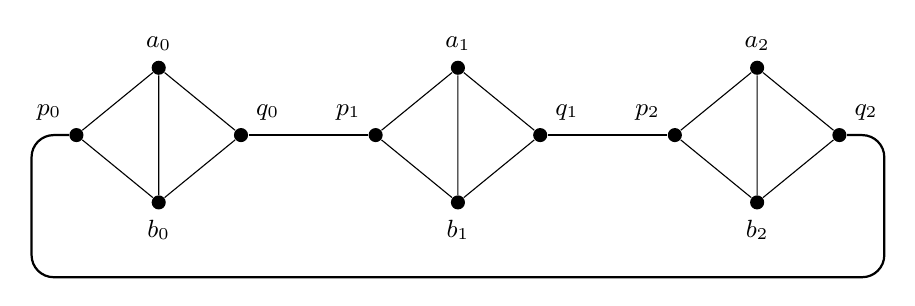
\begin{tikzpicture}[scale=0.95,every node/.style={font=\small},
 point/.style={circle,fill=black,inner sep=1.8pt}]
\foreach \i/\x in {0/0,1/4,2/8} {
 \node[point,label=above:{$a_{\i}$}] (a\i) at (\x,0.9) {};
 \node[point,label=below:{$b_{\i}$}] (b\i) at (\x,-0.9) {};
 \node[point,label=above left:{$p_{\i}$}] (p\i) at (\x-1.1,0) {};
 \node[point,label=above right:{$q_{\i}$}] (q\i) at (\x+1.1,0) {};
 \draw (a\i)--(b\i) (a\i)--(p\i) (a\i)--(q\i)
       (b\i)--(p\i) (b\i)--(q\i);
}
\draw[thick] (q0)--(p1) (q1)--(p2);
\draw[thick,rounded corners=8pt] (q2)--(9.7,0)--(9.7,-1.9)
  --(-1.7,-1.9)--(-1.7,0)--(p0);
\end{tikzpicture}
\caption{The core \(D_3\). Each of its twelve vertices is replaced by
a triangle to obtain \(G_3\). The displayed diamonds are in the core,
not in the 36-vertex expansion.}\label{fig:core}
\end{figure}

\section{A necessary condition on the core}

An external private neighbor of \(v\) with respect to a set \(I\)
is a vertex \(w\in\NN_D(v)\setminus I\) satisfying
\(\NN_D(w)\cap I=\{v\}\). We use this standard terminology only for
the explicitly stated condition below; no domination theorem is
invoked.

\begin{proposition}\label{prop:necessary}
If \(\Exp(D)\) admits a \(\palette\)-packing coloring, then \(D\)
admits a proper three-coloring \(f:\V(D)\to\high\) such that each
vertex of \(I=f^{-1}(C)\) has an external private neighbor with
respect to \(I\).
\end{proposition}

\begin{proof}
Let \(c\) be any \(\palette\)-packing coloring of \(\Exp(D)\).
All labels have positive radius, so adjacent vertices have distinct
labels. In particular, the triangle \(T_v\) cannot be colored solely
with the two labels \(1_a,1_b\). Choose a vertex \(x_v\in T_v\)
having a high label, and put \(f(v)=c(x_v)\).
The choice can be arbitrary; \(T_v\) may contain more than one
high-colored vertex.

If \(uv\in\E(D)\), the triangles \(T_u,T_v\) are disjoint, and
Lemma~\ref{lem:metric} gives \(\dist_{\Exp(D)}(x_u,x_v)\leq3\).
Each high label has radius at least three. Therefore \(f(u)\ne f(v)\),
and \(f\) is proper.

Take \(v\in I\) and write its selected incidence as \(x_v=(v,w)\).
Then \(w\in\NN_D(v)\), and properness shows \(w\notin I\).
Also \(v\in\NN_D(w)\cap I\). If another vertex
\(u\in\NN_D(w)\cap I\), \(u\ne v\), existed, then
Lemma~\ref{lem:metric} and \eqref{eq:fourwalk} would give
\(\dist_{\Exp(D)}(x_v,x_u)\leq4\).
But these are distinct vertices both assigned the label \(C\), whose
radius is four. The required strict inequality is impossible.
Thus \(\NN_D(w)\cap I=\{v\}\), as required.
\end{proof}

\begin{remark}\label{rem:necessity}
Proposition~\ref{prop:necessary} is a necessary condition, not an
equivalence or a coloring algorithm. It neither constructs the
radius-three representatives nor ensures that the remaining vertices
can be colored by the two low labels. The contradiction below needs
only necessity. In particular, no restriction to colorings with
exactly one high vertex per triangle is justified or used.
\end{remark}

\section{The obstruction in odd diamond rings}

\begin{lemma}\label{lem:diamond}
Let \(f\) be a proper three-coloring of \(D_k\) with labels \(A,B,C\).
For each \(i\), the tips \(p_i,q_i\) have a common color \(t_i\),
and \(t_i\ne t_{i+1}\). If every \(C\)-colored vertex has an external
private neighbor with respect to \(f^{-1}(C)\), then \(t_i\ne C\)
for every \(i\).
\end{lemma}

\begin{proof}
The adjacent bases \(a_i,b_i\) have different colors. Each tip is
adjacent to both bases, so both tips have the third color, denoted
by \(t_i\). The joining edge \(q_ip_{i+1}\) gives
\(t_i\ne t_{i+1}\).

Suppose that \(t_i=C\), and put \(I=f^{-1}(C)\). Both \(p_i\)
and \(q_i\) belong to \(I\). By \eqref{eq:tipneighbors}, a possible
private neighbor of \(p_i\) must be one of
\(a_i,b_i,q_{i-1}\). Neither \(a_i\) nor \(b_i\) is private, since
each is also adjacent to \(q_i\in I\), and \(q_i\ne p_i\).

The remaining candidate is \(q_{i-1}\). Its color is
\(t_{i-1}\ne t_i=C\), because \(q_{i-1}p_i\) is an edge.
In the preceding diamond, the two base colors and its tip color are
all three labels. Consequently one of \(a_{i-1},b_{i-1}\) has color
\(C\). This base vertex is adjacent to \(q_{i-1}\), belongs to
\(I\), and is distinct from \(p_i\). Hence \(q_{i-1}\) is not a
private neighbor either. We have exhausted all three neighbors of
\(p_i\), a contradiction.
\end{proof}

\begin{proof}[Proof of Theorem~\ref{thm:main}]
The graph-theoretic assertions follow from Lemma~\ref{lem:structure}.
Suppose \(G_k\) admitted a \(\palette\)-packing coloring.
Proposition~\ref{prop:necessary} would give a proper core
three-coloring with the private-neighbor property.
Lemma~\ref{lem:diamond} would then give labels \(t_i\in\{A,B\}\)
with \(t_i\ne t_{i+1}\) at every cyclic index. Starting with \(t_0\),
these labels alternate around the ring. Since \(k\) is odd,
\(t_{k-1}=t_0\), contradicting the last joining edge.
Thus no such packing coloring exists.
\end{proof}

\begin{remark}[Why radius four matters]
The walk \eqref{eq:fourwalk} has length at most four. For a
radius-three label, this upper bound alone gives no contradiction:
distance four is allowed. The private-neighbor conclusion for \(C\)
therefore uses precisely the stronger distance requirement. By the
known \(\weakpalette\)-colorability result~\cite[Theorem~4]{MEAH},
the members of our family do admit the weaker sequence. This is a
comparison with that theorem, not a new proof of it.
\end{remark}

\section{The fixed certificate and formal verification}

The full mathematical proof above is independent of computation.
For a reproducible finite witness, we additionally specify \(G_3\)
as follows. Number the core vertices by
\[
 a_i=4i,\qquad b_i=4i+1,\qquad p_i=4i+2,\qquad q_i=4i+3
 \quad(0\leq i<3).
\]
List the incidences \((v,w)\) lexicographically, with neighbors of
each \(v\) in increasing numerical order. Number them \(0,\ldots,35\).
This convention determines the graph exactly, without relying on a
picture or a stored distance table.

\subsection{What the Lean theorem proves}

The source \texttt{ClawFree11334.lean} implements this graph as a
Mathlib \texttt{SimpleGraph (Fin 36)}. It proves agreement with the
54 undirected certificate edges, degree exactly three at every
vertex, connectedness by actual walks, exclusion of every induced
claw, and nonisomorphism to every graph on 12 vertices.

The packing predicate is a strict inequality between the radius
\(1,1,3,3,4\) of a label and the actual Mathlib extended graph
distance. The main declaration is
\begin{center}
\texttt{ClawFree11334.original\_counterexample}.
\end{center}
It includes the failure of all color functions
\(\mathrm{Fin}(36)\to\mathrm{Fin}(5)\), not merely failure within a
selected family of colorings. Intermediate declarations establish
the actual length-three and length-four walks, extract arbitrary
high representatives, and prove the core obstruction structurally.
Small ordinary kernel decisions check fixed graph data and local
three-color identities. The proof does not enumerate all five-color
functions, use \texttt{native\_decide}, admit a proof, or introduce
a nonstandard axiom.

The supplied audit covers 18 declarations. Its allowed axioms are
\begin{center}\small
\texttt{propext}, \texttt{Classical.choice}, \texttt{Quot.sound}.
\end{center}
The supplement binds the source, toolchain and actual compilation
log by SHA256. The precise formalization boundary is important:
the Lean theorem covers \(k=3\), and does not formalize all odd
\(k\), or the separate diamond-free observation in
Lemma~\ref{lem:structure}.

\subsection{Reproducibility and independent checks}

The supplement contains the fixed adjacency certificate, the exact
Lean source, version information, and definition-first Python
checks. Our bounded replay reconstructs the incidence graph from
\eqref{eq:coreedges}, compares it with the frozen certificate,
computes full-graph BFS distances, and checks the short-walk bounds.
It includes damaged-input and positive controls, as described in
Appendix~\ref{app:replay}.

An earlier author's exhaustive projected check is retained as
historical evidence: it examined \(3^{12}=531441\) assignments,
found 48 proper core labelings, and checked 3888 candidate selections
for their radius-four representatives, finding none. These figures
are explicitly author-provenanced and are not described as a new
run during manuscript preparation. Neither Theorem~\ref{thm:main}
nor its Lean instance depends on that finite search.

An independent AI reviewer, uninvolved in discovery, implementation
and manuscript writing, rederived the proof from the original
definitions and checked the manuscript's mathematical and semantic
claims. AI-assisted independent checking is not external human peer
review. Version-bound review and execution records are included with
the private manuscript materials.

\section{Discussion}

The obstruction has two distinct components. Triangle expansion
converts short walks into restrictions on a core coloring. The
diamond ring then amplifies the local private-neighbor restriction
into a global parity contradiction. This explains why the witness
extends to arbitrarily large orders without a search or a new
distance calculation for each graph.

The core condition is a useful way to test a proposed
\(\palette\)-coloring route, but we have not proved that it is
sufficient. Even ring lengths escape the final parity contradiction;
that fact alone does not prove their expanded graphs colorable.
An explicit \(k=4\) coloring is checked as a positive control in
the supplement. We do not claim a classification of all admissible
cores, the smallest counterexample, or a solution to other packing
coloring problems.

The fixed formal witness is enough to give a negative answer to
the original universal question. Extending the Lean development
to cyclic indices of arbitrary odd order would formalize the
family theorem, but is not needed for the mathematical proof
presented here. The source's positive results for weaker palettes
remain part of the existing literature and are not counted as
additional new results of this paper.

\section*{AI assistance and responsibility}

AI agents assisted the project's mathematical exploration, proof
derivation, Lean implementation, code checking and technical writing.
For this manuscript an additional AI reviewer independently examined
the original statement, the family proof and the formalization's
scope. This disclosure does not assert a human-only research process
or external human peer review. No AI system is listed as an author.
Human authorship, contribution statements and final responsibility
review remain to be confirmed for this private draft. Funding,
conflict-of-interest, correspondence and license declarations are
also pending; no declaration is inferred from an earlier paper.

\appendix
\section{Exact replay and certificate conventions}\label{app:replay}

The fixed JSON certificate uses the numbering given in Section~6.
Undirected edge pairs are stored once, with the smaller endpoint
first, in lexicographic order. The incidence labels and the palette
are part of the certificate, not descriptive metadata that a checker
may ignore. The following pseudocode reconstructs the object.
\begin{quote}\small
For each cyclic index \(i\), add the five diamond edges and
\(q_ip_{i+1}\). For each core vertex \(v\), sort its three neighbors
and list the incidences \((v,w)\). Join all three pairs within
\(T_v\), and join each incidence to its reciprocal \((w,v)\).
Reject loops, repeated edges and a mismatching certificate. Compute
BFS from every expanded vertex.
\end{quote}

The bounded structural replay checks cubicity, connectivity,
claw-freeness, unique replacement triangles, and all the metric
bounds used in Proposition~\ref{prop:necessary}. It checks the
tip-neighbor formulas at every cyclic index without enumerating
the full space of original colorings. A separate independent checker
reconstructs the graph without importing the author's verifier.
The finite regressions are checks of the implementation, not proofs
of the all-odd-\(k\) statement.

The controls include a missing edge, a corrupted incidence label,
a changed palette, an invalid equal-low-label coloring on adjacent
vertices, a valid \(\weakpalette\) coloring of \(G_3\), and a valid
\(\palette\) coloring of \(G_4\). Every positive coloring is tested
against distances in the entire expanded graph. The historical
exhaustive verifier remains available as an optional command; it is
not part of the bounded publication replay.

For Lean, use the supplied \texttt{lean-toolchain} and
\texttt{lake-manifest.json}; the evidence uses Lean 4.34.1 and
Mathlib commit
\begin{center}\small\texttt{d13f23b723b8a846827a245b89c10fc7d3f11612}.\end{center}
The \texttt{REPRODUCE.md} file gives the exact commands, including
the standalone source-root option. The delivery manifest binds the
paper, source, certificate, reviews and execution records by SHA256.
Installing Lean from an empty cache is a separate environment step
and is not claimed as a tested part of this package replay.

\begin{thebibliography}{9}
\small
\raggedright

\bibitem{AKM}
S.~E. Anderson, K. Kuenzel and J.~D. Marcano Cuellar,
\emph{Diamond-free, claw-free cubic graphs are
\((1,1,2,3)\)-packing colorable},
arXiv:2607.25198v1 (2026).
\url{https://arxiv.org/abs/2607.25198}.

\bibitem{BKR}
B. Bre\v{s}ar, K. Kuenzel and D.~F. Rall,
\emph{Claw-free cubic graphs are \((1,1,2,2)\)-colorable},
Discrete Mathematics \textbf{348} (2025), article 114477;
preprint arXiv:2409.15455v1.
\url{https://arxiv.org/abs/2409.15455}.

\bibitem{survey}
B. Bre\v{s}ar, J. Ferme, S. Klav\v{z}ar and D.~F. Rall,
\emph{A survey on packing colorings},
Discussiones Mathematicae Graph Theory \textbf{40} (2020), 923--970.
\url{https://doi.org/10.7151/dmgt.2320}.

\bibitem{GT}
N. Gastineau and O. Togni,
\emph{\(S\)-packing colorings of cubic graphs},
Discrete Mathematics \textbf{339} (2016), 2461--2470;
preprint arXiv:1403.7495.
\url{https://arxiv.org/abs/1403.7495}.

\bibitem{MEAH}
M. Mortada, A. El Zein and S. Al Hajjar,
\emph{On \((1,1,2,3)\)- and \((1,1,3,3,3)\)-packing colorings
of claw-free subcubic graphs},
arXiv:2608.02566v1 (2026), Section~6, Problem~1.
\url{https://arxiv.org/html/2608.02566v1#S6}.

\bibitem{MEZ}
M. Mortada and A. El Zein,
\emph{A short proof that every claw-free cubic graph is
\((1,1,2,2)\)-packing colorable},
Discrete Applied Mathematics \textbf{391} (2026), 24--27;
preprint arXiv:2512.24001v1.
\url{https://arxiv.org/abs/2512.24001}.

\bibitem{Oum}
S.-il Oum, \emph{Perfect matchings in claw-free cubic graphs},
Electronic Journal of Combinatorics \textbf{18} (2011), \#P62.
\url{https://doi.org/10.37236/549}.

\end{thebibliography}
\end{document}
